\onehalfspacing
\section{Đề số 20}
\graphicspath{{./img/}}
\begin{bt} 
    \hfil
    \begin{enumerate}[a.]
        \item Tính $M=\left(\frac{0,4-\frac{2}{9}+\frac{2}{11}}{1,4-\frac{7}{9}+\frac{7}{11}}-\frac{\frac{1}{3}-0,25+\frac{1}{5}}{1 \frac{1}{6}-0,875+0,7}\right): \frac{2017}{2018}$.
        \item Tìm x, biết: $|2017-x|+|2018-x|+|2019-x|=2$.
    \end{enumerate}
\loigiai{
    \begin{enumerate}
        \item $\text {Ta có: } M=\left(\frac{0,4-\frac{2}{9}+\frac{2}{11}}{1,4-\frac{7}{9}+\frac{7}{11}}-\frac{\frac{1}{3}-0,25+\frac{1}{5}}{1 \frac{1}{6}-0,875+0,7}\right): \frac{2017}{2018} \\[5px]
        =\left(\frac{\frac{2}{5}-\frac{2}{9}+\frac{2}{11}}{\frac{7}{5}-\frac{7}{9}+\frac{7}{11}}-\frac{\frac{1}{3}-\frac{1}{4}+\frac{1}{5}}{\frac{7}{6}-\frac{7}{8}+\frac{7}{10}}\right): \frac{2017}{2018} \\[5px]
        =\left(\frac{2\left(\frac{1}{5}-\frac{1}{9}+\frac{1}{11}\right)}{7\left(\frac{1}{5}-\frac{1}{9}+\frac{1}{11}\right)}-\frac{\left(\frac{1}{3}-\frac{1}{4}+\frac{1}{5}\right)}{\frac{7}{2}\left(\frac{1}{3}-\frac{1}{4}+\frac{1}{5}\right)}\right): \frac{2017}{2018} \\[5px]
        =\left(\frac{2}{7}-\frac{2}{7}\right): \frac{2017}{2018}=0 \\[5px]$
        \item Có $|2018-x| \geq 0$ và
        $|2017-x|+|2019-x|=|x-2017|+|2019-x| \geq|x-2017+2019-x|=2 \\[5px]
        \Rightarrow|2017-x|+|2018-x|+|2019-x| \geq 2$\\[5px]
        Dấu "=" xảy ra khi và chi khi $(x-2017)(2019-x) \geq 0$ và $2018-x=0$, suy ra: $2017 \leq x \leq 2019$ và $\mathrm{x}=2018 \Rightarrow \mathrm{x}=2018$\\[5px]
        Vậy $x=2018$.
    \end{enumerate}
}
\end{bt}

\begin{bt}
    \hfill
	\begin{enumerate}[a.]
        \item Cho a, b, c là ba số thực dương thỏa mãn điều kiện:
        $$
        \frac{\mathrm{a}+\mathrm{b}-\mathrm{c}}{\mathrm{c}}=\frac{\mathrm{b}+\mathrm{c}-\mathrm{a}}{\mathrm{a}}=\frac{\mathrm{c}+\mathrm{a}-\mathrm{b}}{\mathrm{b}}
        $$
        Hãy tính giá trị của biểu thức: $\mathrm{B}=\left(1+\frac{\mathrm{b}}{\mathrm{a}}\right)\left(1+\frac{\mathrm{a}}{\mathrm{c}}\right)\left(1+\frac{\mathrm{c}}{\mathrm{b}}\right)$.
        \item Cho hai đa thức: $f(x)=(x-1)(x+3)$ và $g(x)=x^3-a x^2+b x-3$
        Xác định hệ số $a$; b của đa thức $\mathrm{g}(\mathrm{x})$ biết nghiệm của đa thức $\mathrm{f}(\mathrm{x})$ cũng là nghiệm của đa thức $\mathrm{g}(\mathrm{x})$.
        \item Tìm các số nguyên dương $x, y$, $z$ thỏa mãn: $x+y+z=x y z$.
    \end{enumerate}
	\loigiai{
        \begin{enumerate}
            \item Vì a, b,c là các số dương nên $a+b+c \neq 0$\\[5px]
            Nên theo tính chất dãy tỉ số bằng nhau ta có:\\[5px]
            $\frac{a+b-c}{c}=\frac{b+c-a}{a}=\frac{c+a-b}{b}=\frac{a+b-c+b+c-a+c+a-b}{a+b+c}=1 \\[5px]
            \Rightarrow \frac{a+b-c}{c}+1=\frac{b+c-a}{a}+1=\frac{c+a-b}{b}+1=2 \\[5px]
            \Rightarrow \frac{a+b}{c}=\frac{b+c}{a}=\frac{c+a}{b}=2 \\[5px]
            \text {Mà: } B=\left(1+\frac{b}{a}\right)\left(1+\frac{a}{c}\right)\left(1+\frac{c}{b}\right) \\[5px]
            \Rightarrow B=\left(\frac{a+b}{a}\right)\left(\frac{c+a}{c}\right)\left(\frac{b+c}{b}\right)=8\\[5px] 
            \text{Vậy } B = 8$
            \item HS biết tìm nghiệm của $f(x)=(x-1)(x+3)=0 \Leftrightarrow x=1 ; x=-3$\\[5px]
            Nghiệm của $f(x)$ cũng là nghiệm của $g(x)=x^3-a x^2+b x-3$ nên:\\[5px]
            Thay $\mathrm{x}=1$ vào $\mathrm{g}(\mathrm{x})$ ta có: $1-\mathrm{a}+\mathrm{b}-3=0$\\[5px]
            Thay $x=-3$ vào $g(x)$ ta có: $-27-9 a-3 b-3=0$\\[5px]
            Từ đó $\mathrm{HS}$ biến đổi và tính được: $\mathrm{a}=-3 ; \mathrm{b}=-1$
            \item Vì $x, y, z \in Z^{+}$nên giả sử $1 \leq x \leq y \leq z$\\[5px]
            Theo bài ra: $1=\frac{1}{\mathrm{yz}}+\frac{1}{\mathrm{yx}}+\frac{1}{\mathrm{zx}} \leq \frac{1}{\mathrm{x}^2}+\frac{1}{\mathrm{x}^2}+\frac{1}{\mathrm{x}^2}=\frac{3}{\mathrm{x}^2}$\\[5px]
            Suy ra: $x^2 \leq 3 \Rightarrow x=1$\\[5px]
            Thay vào đầu bài ta có:\\[5px]
            $1+y+z=y z \Rightarrow y-y z+1+z=0 \\[5px]
            \Rightarrow y(1-z)-(1-z)+2=0 \\[5px]
            \Rightarrow(y-1)(z-1)=2$\\[5px]
            TH1: $\left\{\begin{array}{l}\mathrm{y}-1=1 \\[5px] z-1=2\end{array} \Rightarrow\left\{\begin{array}{l}\mathrm{y}=2 \\[5px] z=3\end{array}\right.\right.$\\[5px]
            TH2: $\left\{\begin{array}{l}y-1=2 \\[5px] z-1=1\end{array} \Rightarrow\left\{\begin{array}{l}y=3 \\[5px] z=2\end{array}\right.\right.$ (loại)\\[5px]
            Vậy $(x ; y ; z)=(1 ; 2 ; 3)$ và các hoán vị
        \end{enumerate}
    } 
\end{bt}

\begin{bt}
    Cho tam giác $\mathrm{ABC}$ cân tại $\mathrm{A}, \mathrm{BH}$ vuông góc $\mathrm{AC}$ tại $\mathrm{H}$. Trên cạnh $\mathrm{BC}$ lấy điểm $\mathrm{M}$ bất kì ( $M$ khác $B$ và $C)$. Gọi $D, E, F$ là chân đường vuông góc hạ từ $M$ đến $A B, A C, B H$.
	\begin{enumerate}[a.]
        \item Chứng minh: $\triangle \mathrm{DBM}=\triangle \mathrm{FMB}$.
        \item Chứng minh khi $M$ chạy trên cạnh $\mathrm{BC}$ thì tổng $\mathrm{MD}+\mathrm{ME}$ có giá trị không đổi.
        \item Trên tia đối của tia $CA$ lấy điểm $\mathrm{K}$ sao cho $\mathrm{CK}=\mathrm{EH}$.
        Chứng minh $\mathrm{BC}$ đi qua trung điêm của đoạn thẳng $\mathrm{DK}$.
    \end{enumerate}
	\loigiai{
        $$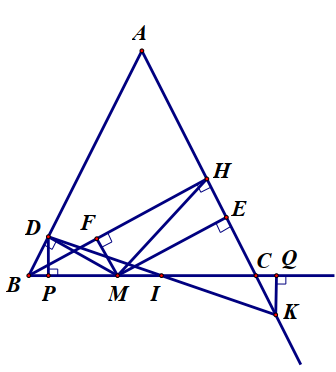
\includegraphics[width=0.4\textwidth]{20-3-lg.png}$$
        \begin{enumerate}
            \item Chứng minh được $\Delta \mathrm{DBM}=\Delta F M B$ (ch-gn)
            \item Theo câu a ta có: $\triangle \mathrm{DBM}=\Delta \mathrm{FMB}$ (ch-gn) $\Rightarrow \mathrm{MD}=\mathrm{BF}$ (2 cạnh tương ứng)$(1)$\\[5px]
            +) $\mathrm{C} / \mathrm{m}: \Delta \mathrm{MFH}=\Delta \mathrm{HEM} \Rightarrow \mathrm{ME}=\mathrm{FH}$ (2 cạnh tương ứng)$(2)$\\[5px]
            Từ (1) và (2) suy ra: $\mathrm{MD}+\mathrm{ME}=\mathrm{BF}+\mathrm{FH}=\mathrm{BH}$\\[5px]
            BH không đổi $\Rightarrow M D+M E$ không đổi (đpcm)
            \item Vẽ $\mathrm{DP} \perp \mathrm{BC}$ tại $P, K Q \perp B C$ tại $Q$, gọi $\mathrm{I}$ là giao điểm của $\mathrm{DK}$ và $B C$\\[5px]
            +) Chứng minh: $\mathrm{BD}=\mathrm{FM}=\mathrm{EH}=\mathrm{CK}$\\[5px]
            +) Chứng minh: $\triangle \mathrm{BDP}=\Delta \mathrm{CKQ}$(ch-gn) $\Rightarrow \mathrm{DP}=\mathrm{KQ}$ (cạnh tương ứng)\\[5px]
            +) Chứng minh: $\mathrm{IDP}=\mathrm{IKQ} \Rightarrow \Delta \mathrm{DPI}=\Delta \mathrm{KQI}(\mathrm{g}-\mathrm{c}-\mathrm{g}) \Rightarrow \mathrm{ID}=\mathrm{IK}(\text{đpcm})$
        \end{enumerate}
    }
\end{bt}

\begin{bt}
    Cho tam giác $A B C\left(A B<A C, B=60^{\circ}\right)$. Hai tia phân giác $A D$ $(D \in B C)$ và $C E$ ( $\mathrm{E} \in \mathrm{AB}$ ) của $\triangle \mathrm{ABC}$ cắt nhau ở I. Chứng minh $\Delta \mathrm{IDE}$ cân.
\loigiai{
    $$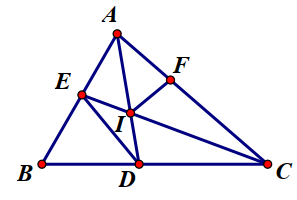
\includegraphics[width=0.4\textwidth]{20-4-lg.png}$$
    Ta có $\mathrm{ABC}=60^{\circ} \Rightarrow \mathrm{BAC}+\mathrm{BCA}=120^{\circ}$\\[5px]
    $\mathrm{AD}$ là phân giác của $\mathrm{BAC}$ suy ra $\mathrm{IAC}=\frac{1}{2} \mathrm{BAC}$\\[5px]
    $\mathrm{CE}$ là phân giác của $\mathrm{ACB}$ suy ra $\mathrm{ICA}=\frac{1}{2} \mathrm{BCA}$\\[5px]
    Suy ra $\mathrm{IAC}+\mathrm{ICA}=\frac{1}{2} \cdot 120^{\circ}=60^{\circ} \Rightarrow \mathrm{AIC}=120^{\circ}$\\[5px]
    Do đó $\mathrm{AIE}=\mathrm{DIC}=60^{\circ}$\\[5px]
    Trên cạnh $\mathrm{AC}$ lấy điểm $\mathrm{F}$ sao cho $\mathrm{AF}=\mathrm{AE}$\\[5px]
    Xét $\triangle \mathrm{EAI}$ và $\triangle \mathrm{FAI}$ có:\\[5px]
    $\mathrm{AE}=\mathrm{AF}$\\[5px]
    $\mathrm{EAI}=\mathrm{FAI}$\\[5px]
    $AI$ chung\\[5px]
    Vậy $\Delta \mathrm{EAI}=\Delta \mathrm{FAI}(\mathrm{c}-\mathrm{g}-\mathrm{c})$\\[5px]
    suy ra IE =IF (hai cạnh tương ứng) (1)\\[5px]
$\mathrm{AIE}=\mathrm{AIF}=60^{\circ} \Rightarrow \mathrm{FIC}=\mathrm{AIC}-\mathrm{AIF}=60^{\circ}$\\[5px]
Chứng minh $\Delta \mathrm{DIC}=\Delta \mathrm{FIC}(\mathrm{g}-\mathrm{c}-\mathrm{g})$\\[5px]
Suy ra $\mathrm{ID}=\mathrm{IF}$ (hai cạnh tương ứng) (2)\\[5px]
Từ (1) và (2) suy ra $\Delta \mathrm{IDE}$ cân tại I
}
\end{bt}

\begin{bt}
    Cho $\operatorname{S}_{\mathrm{n}}=\frac{1^2-1}{1}+\frac{2^2-1}{2^2}+\frac{3^2-1}{3^2}+\ldots+\frac{\mathrm{n}^2-1}{\mathrm{n}^2}$ (với $\mathrm{n} \in \mathrm{N}$ và $\mathrm{n}>1$ )
    
    Chứng minh rằng $\mathrm{S}_{\mathrm{n}}$ không là số nguyên.
    \loigiai{
    $\text { Có } S_n=1-\frac{1}{1^2}+1-\frac{1}{2^2}+1-\frac{1}{3^2}+\ldots+1-\frac{1}{n^2} \\[5px]
    =(n-1)-\left(\frac{1}{2^2}+\frac{1}{3^2}+\ldots+\frac{1}{n^2}\right)$\\[5px]
    Đặt $\mathrm{A}=\frac{1}{2^2}+\frac{1}{3^2}+\ldots+\frac{1}{\mathrm{n}^2}$\\[5px]
    Do $\mathrm{A}>0$ nên $\mathrm{S}_{\mathrm{n}}<\mathrm{n}-1$\\[5px]
    Mặt khác $\mathrm{A}<\frac{1}{1.2}+\frac{1}{2.3}+\ldots+\frac{1}{(\mathrm{n}-1) \cdot \mathrm{n}}=1-\frac{1}{\mathrm{n}}$\\[5px]
    $\Rightarrow \mathrm{S}_{\mathrm{n}}>(\mathrm{n}-1)-\left(1-\frac{1}{\mathrm{n}}\right)=\mathrm{n}-2+\frac{1}{\mathrm{n}}>\mathrm{n}-2\left(\text { do } \frac{1}{\mathrm{n}}>0\right)$\\[5px]
    $\Rightarrow \mathrm{n}-2<S_n<n-1$ nên $S_n$ không là số nguyên
    }
\end{bt}

